\section{Introduzione}
Per rendere maggiormente leggibile il codice Matlab e, allo stesso tempo, ridurre i tempi necessari per l'esecuzione, abbiamo deciso di dividere le varie funzionalità in diversi \textit{livescript}: in particolar modo la parte relativa allo studio ed alla definizione del controllore siamo andati ad inserirla all'interno del file \textit{GainCalculator.mlx} dove si può vedere che le prime istruzioni vanno a caricare dal workspace, risultante dalla precedente linearizzazione, le matrici A-B-C-D che definiscono il sistema lineare modellizzato.

\section{Analisi in anello aperto}
\label{sec:open_loop_analysis}
Prima di procedere con l'individuazione del controllore più adatto per stabilizzare il V.A.B., siamo andati ad effettuare una breve analisi sul sistema ad anello aperto, per ottenere così alcuni spunti sulla correttezza del modello che era stato steso fino a quel punto.

Come noto dalla teoria, il sistema risulta essere asintoticamente stabile se gli autovalori della matrice A risultano avere tutti parte reale negativa; è instabile invece se è presente almeno un autovalore con parte reale strettamente positiva.

Abbiamo quindi calcolato gli autovalori con il comando seguente:
\begin{lstlisting} [caption={Calcolo autovalori matrice A (non simbolica)},captionpos=b]
eig(A_real)
\end{lstlisting}

La presenza di autovalori con parte reale strettamente positiva è stata confermata anche dalla visualizzazione del luogo delle radici (\textit{rlocus}) del sistema in anello aperto: come si vede in figura ~\ref{fig:r_locus_openloop}, il polo che si trova nel semi-piano reale positivo non potrà, in alcun modo, essere stabilizzato, ovvero portato nel semi-piano sinistro.

Questa breve analisi ci ha permesso di avere una conferma numerica del fatto ovvio che, senza un controllo, il V.A.B. in esame non riesce a mantenere da solo la posizione verticale.

\begin{figure}[H]
	\centering   	
	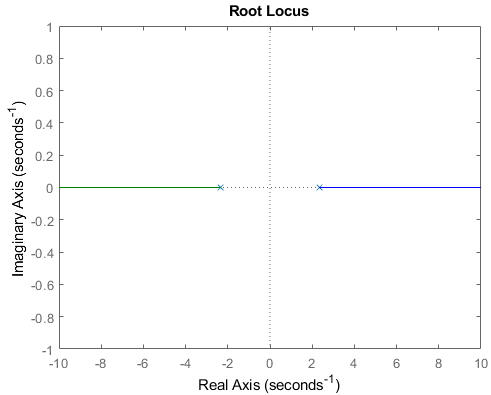
\includegraphics[width=0.5\textwidth]{Immagini/root_locus_open_loop.png}
	\caption{Luogo delle radici del V.A.B. modellizzato in anello aperto}
	\label{fig:r_locus_openloop}
\end{figure}

\begin{figure}[H]
	\centering   	
	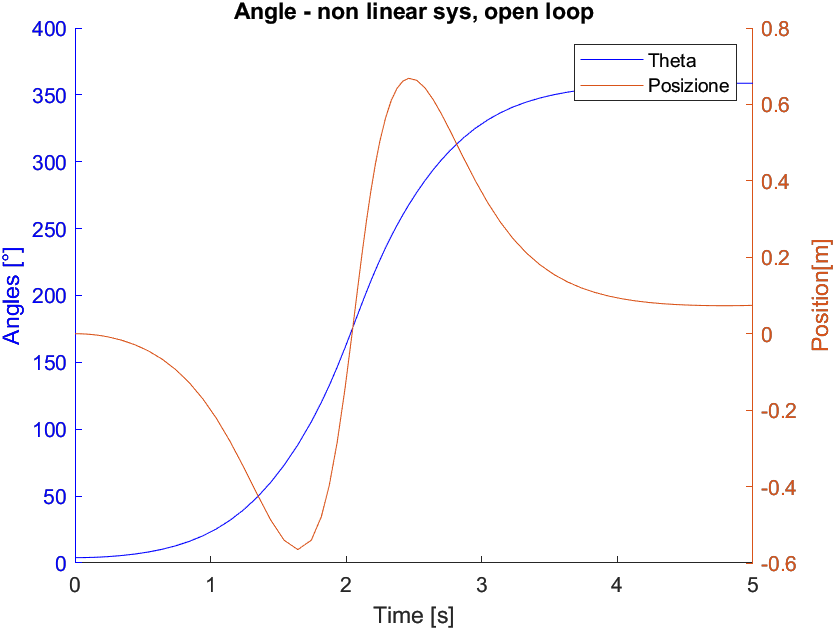
\includegraphics[width=0.5\textwidth]{Immagini/open_loop_response_non_linear.png}
	\caption{Risposta del sistema non lineare in anello aperto}
	\label{fig:openloop_nonlin_response}
\end{figure}

\section{Controllore}
Per quanto riguarda il sistema del veicolo autobilanciato, siamo andati a far riferimento a quella classe di problemi definiti come \textit{problemi di regolazione}, in cui il sistema si presenta inizialmente con una condizione iniziale dello stato non nulla, condizione che si intende di riportare a zero con una velocità di convergenza assegnata.

Nello specifico, questo tipo di problema relativo alla scelta del controllore, è stato risolto mediante l'utilizzo dell'assegnazione degli autovalori ottenuti tramite retroazione dello stato, in cui il moto del sistema è composto completamente dal moto libero che si vuole controllare e annullare in un tempo a piacere.

Il posizionamento dei poli, e quindi la scelta del guadagno del regolatore, va eseguita sul solo sistema lineare: questo a conferma sia di quanto riportato in figura ~\ref{fig:feedback_state} (nel blocco di colore blu infatti è riportato il sistema lineare), sia di quanto detto in precedenza in merito al fatto che il controllore venga ad essere definito lavorando sul sistema linearizzato.

\begin{figure}[H]
	\centering   	
	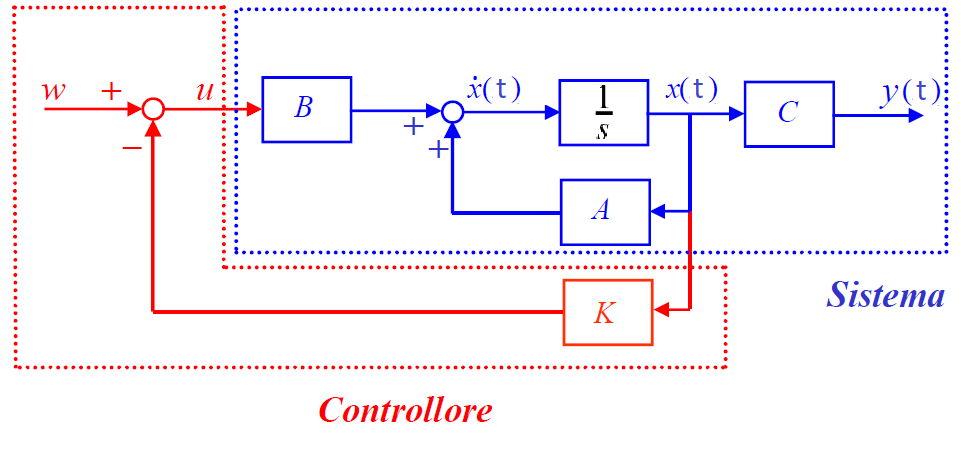
\includegraphics[width=0.70\textwidth]{Immagini/feedback_state.png}
	\caption{Schema concettuale del controllo (\cite{feedback_state})}
	\label{fig:feedback_state}
\end{figure}

Ciò che è riportato graficamente in figura \ref{fig:feedback_state}, può essere riscritto matematicamente come segue:
\begin{center}
	$
	\begin{cases}
	\begin{array}{c}
	\dot{x}\left(t\right)=Ax{\left(t\right)}+Bu\left(t\right)\\
	y{\left(t\right)}=Cx{\left(t\right)}+Du\left(t\right)
	\end{array}
	\end{cases}
	$
	$$
	u{\left(t\right)}=-Kx{\left(t\right)}+w{\left(t\right)}	= \text{ legge di controllo}
	$$
\end{center}

Dunque, sostituendo la legge di controllo nell'equazione di stato del sistema, possiamo ottenere le seguenti equazioni che ci permettono di definire il legame del sistema in anello chiuso con la matrice K:
\begin{center}
	$
	\dot{x}{\left(t\right)}=Ax{\left(t\right)}+Bu{\left(t\right)}=Ax{\left(t\right)}+B{\left(-Kx{\left(t\right)}+w{\left(t\right)}\right)}
	$
	$$
	=Ax{\left(t\right)}-BKx{\left(t\right)}+Bw\left(t\right)={\left(A-BK\right)}x{\left(t\right)}+Bw{\left(t\right)}
	$$
	$$
	A_{cl} =A-BK = \text{ matrice di stato in anello chiuso (cl $\rightarrow$ closed loop)}
	$$
\end{center}

\subsection{Posizionamento dei poli continui}
Per scegliere il valore da assegnare a K, e quindi definire il guadagno del controllore, è necessario scegliere la posizione desiderata dei poli, in base a quelle che sono le specifiche di velocità desiderate.

\begin{center}
	$
	G{\left(S\right)}=\frac{\omega {\;}_n^{2\;} }{s^2 +2\xi \omega {\;}_n s+\omega {\;}_n^{2\;} }
	$
\end{center}

\begin{center}
	$
	\xi =0\ldotp 7
	$
	$$
	\omega {\;}_{n\;}=2 \pi f_{\mathrm{propria}}
	$$
\end{center}

Dovendo posizionare due coppie di poli complessi coniugati si sono scelte due frequenze ad una decade di distanza, in maniera tale da poter considerare le variabili che sono controllate disaccoppiate in frequenza: essendo il limite di banda (ovvero entro quali limiti il segnale passa senza essere attenuato e/o modificato) del sistema interno molto più alto del limite di banda del sistema esterno, possiamo considerarli disaccoppiati in frequenza.

\begin{center}
	$
	f_{\mathrm{propria\theta}} =  0.2 \text{ Hz}
	$
	$$
	f_{\mathrm{propria\phi}} =  0.02 \text{ Hz}
	$$
\end{center}

Nello specifico, una prima osservazione, è il fatto che il polo più veloce (ovvero quello con frequenza pari a 0.2 Hz) è stato assegnato alla parte relativa al controllo dell'angolo $\theta$, essendo che è auspicabile un controllo maggiormente reattivo per quanto riguarda la stabilizzazione della base, piuttosto che il rapido raggiungimento del set point di posizione spaziale (e quindi angolare $\phi$ delle ruote).

Una seconda osservazione è che, per motivi esterni, il motore risulta avere una coppia massima molto limitata (per via delle limitazioni di corrente): è stato dunque necessario posizionare i poli ad una frequenza tale che permettesso di non saturare per molto tempo la coppia fornita dal motore.
Questa scelta ha inevitabilmente rallentato la risposta del sistema.

Definita quindi la frequenza a cui posizionare i poli, siamo andati a risolvere l'equazione al denominatore della forma generica della f.d.t (G(s)) con due poli complessi: la risoluzione di questa equazione, come è noto dalla teoria, permette di ottenere i valori della variabile di Laplace \textit{s} che azzerano il denominatore stesso, che corrisponde a:

\begin{center}
	$s^2 +2\,\mathrm{\xi}\,s\,{{w_n}} +{{{w_n}}}^2 =0$
\end{center}

Nella nostra simulazione i valori numerici ottenuti per i poli sono stati i seguenti:
\begin{center}
	$
	polo_{\theta} = \left(\begin{array}{c}
	-\frac{7\,\pi }{250}+\frac{\pi \,\sqrt{51}\,\mathrm{i}}{250}\\
	-\frac{7\,\pi }{250}-\frac{\pi \,\sqrt{51}\,\mathrm{i}}{250}
	\end{array}\right)
	$
	$$
	polo_{\phi} = \left(\begin{array}{c}
	-\frac{7\,\pi }{25}+\frac{\pi \,\sqrt{51}\,\mathrm{i}}{25}\\
	-\frac{7\,\pi }{25}-\frac{\pi \,\sqrt{51}\,\mathrm{i}}{25}
	\end{array}\right)
	$$
\end{center}	

Con il comando \textit{place} di Matlab si ottiene dunque:
\begin{center}
	
	$	K =[  -0.0023  , -0.0278, -28.1397  , -7.7022]$
	
\end{center}

Ricordando a questo punto quanto detto nella prima parte di questo capitolo in merito alla definizione della matrice A in anello chiuso, siamo andati a definirla appunto come

\begin{center}
	$
	A_{cl} =A-BK
	$
\end{center}

utilizzando il valore di K appena trovato: una volta trovata la nuova matrice A, siamo andati a ri-effettuare le stesse analisi portate avanti anche per il sistema in anello aperto.

Come si vede in figura ~\ref{fig:closed_loop_root}, grazie al posizionamento degli autovalori, siamo stati in grado di spostare i nuovi poli nel semi-piano sinistro: questo significa quindi che siamo riusciti a stabilizzare il nostro sistema dinamico.
\begin{figure}[H]
	\centering   	
	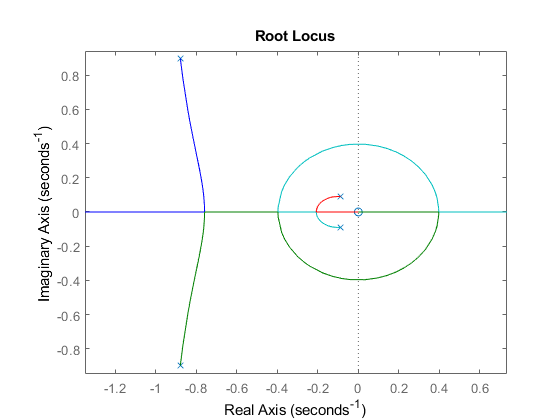
\includegraphics[width=0.7\textwidth]{Immagini/root_locus_closed_loop.png}
	\caption{Root locus del sistema in anello chiuso}
	\label{fig:closed_loop_root}
\end{figure}

\subsection{Setpoint di velocità}
Oltre al controllo del moto libero del sistema è stata implementata anche la possibilità di inserire un setpoint sulla velocità a fine transitorio del Segway. In questo modo si apre la possibilità per l'utente finale di impostare la velocità desiderata e di mantenerla nel tempo nonostante i vari disturbi che in un sistema reale agiranno sulla macchina(vento, salita, discesa..) 
\begin{figure}[H]
	\centering   	
	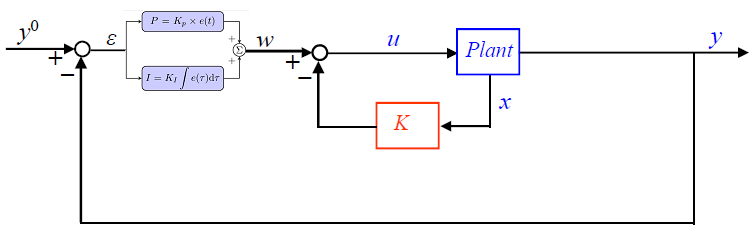
\includegraphics[width=0.8\textwidth]{Immagini/y_setpoint.png}
	\caption{chiusura dell'anello di controllo di $\dot{\phi}$ con un controllore \textit{I} 
	\cite{feedback_state}}
	\label{fig:y_setpoint}
\end{figure}
In figura \ref{fig:y_setpoint} si nota come l'anello di $\dot{\phi}$ sia esterno rispetto all'anello di retroazione dello stato; solitamente si procede dunque nel progettare il controllore avendo cura di lasciare una decade di spazio tra la frequenza del polo dell' integratore e la coppia di poli più lenta del controllore della retroazione dello stato.

In questo caso, per ragioni puramente pratiche, non è stato possibile : il sistema presenta una risposta particolarmente lenta agli input viste le limitazioni di coppia (imposte dai limiti di corrente definiti in fase di specifica del progetto) di cui si approfondirà successivamente.

Sarebbe quindi stato necessario quindi troppo tempo per raggiungere il setpoint di velocità se si fosse proceduto a lasciare una decade di distanza. Si è invece proceduto a posizionare il polo dell'integratore tramite la funzione di Tuning offerta da Matlab Simulink stesso:
\begin{figure}[H]
	\centering   	
	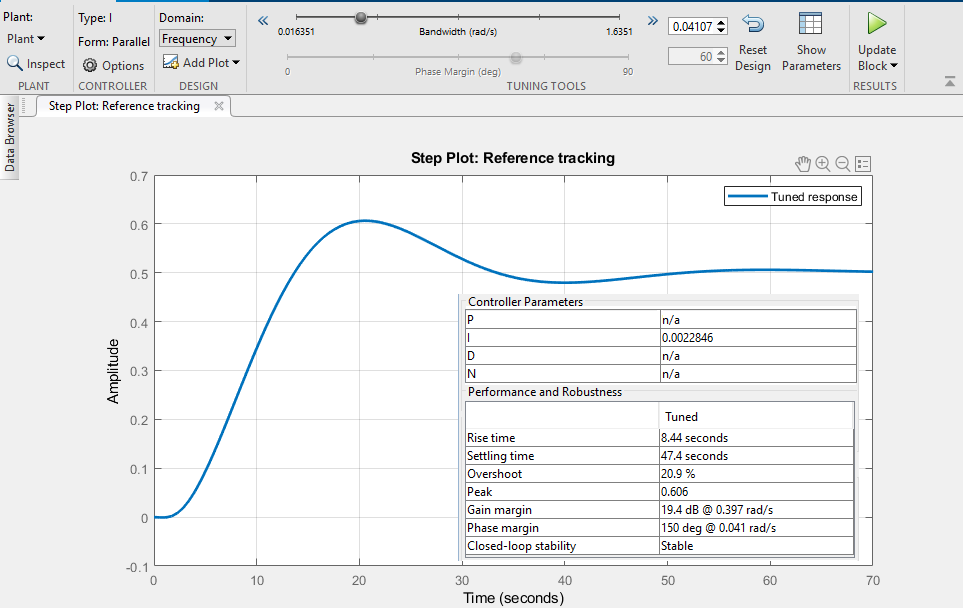
\includegraphics[width=0.75\textwidth]{Immagini/pid_tuning.png}
	\caption{Taratura del controllore}
	\label{fig:pid_tuning}
\end{figure}
Il tuning è stato effettuato sul sistema lineare in quanto Matlab richiede un sistema lineare per questo tipo di tecniche.

Da notare inoltre, in figura \ref{fig:pid_tuning} che la frequenza $f_3 = \dfrac{0.041 \textit{rad/s}}{2\pi} = 0.0065 Hz$ che è circa $\dfrac{1}{3} 	f_{\mathrm{propria\phi}}$.

Sempre in figura \ref{fig:pid_tuning} si osserva che, nonostante non sia stata rispettato la decade di distanza, il sistema sia comunque molto lento e arrivi a regime in circa 70 \textit{s}.

TODO: perchè arriva a 0.5? per la retroazione interna?

\section{OPC - UA}
Per quanto riguarda la parte di controllo, il sistema presenta un controllore centralizzato, rappresentato da un Raspberry: nello specifico ad esso sono affidate delle mansioni ben specifiche, tutte ovviamente volte al controllo e alla stabilizzazione del \textit{veicolo auto bilanciato}.

In questa fase dello sviluppo del progetto, siamo andati ad implementare parte del codice che verrà installato, in un secondo momento, a bordo del Raspberry: esso infatti svolge, all'interno del sistema (come si vede in figura ~\ref{fig:OPCUA_schema}) una comunicazione a due direzioni, che ne determinano due comportamenti differenti:
\begin{itemize}
	\item Come \textbf{server} per la parte di comunicazione \textit{OPC-UA} (per il settaggio dei guadagni) nei confronti di un client (ovvero dell'utente che intende settare i parametri del controllore);
	\item Come \textbf{master} nei confronti della sezione di sensoristica a bordo del V.A.B. (per quanto riguarda invece la gestione dell'algoritmo di controllo);
\end{itemize}

 \begin{figure}[H]
	\centering   	
	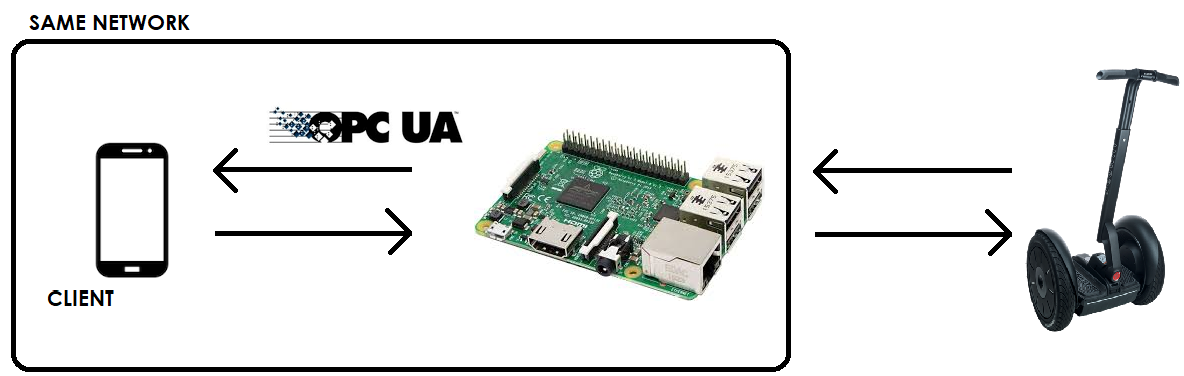
\includegraphics[width=0.75\textwidth]{Immagini/OPCUA_schema.png}
	\caption{Schema di massima dell'utilizzo di Raspberry Pi 3}
	\label{fig:OPCUA_schema}
\end{figure}

In questa fase abbiamo quindi sviluppato la parte relativa all'utilizzo di \textit{Raspberry Pi 3} come \textit{server OPCUA}: in seguito, nella sezione ~\ref{sec:xenomai}, ci occuperemo di andare a rendere Raspberry un controllore Real-Time, tramite il framework \textit{Xenomai}.

\subsection{Idea base OPC-UA}
L'\textit{Open Platform Communications Unified Architecture} (OPC UA) è un protocollo di comunicazione automatico per l'automazione industriale: OPC UA sostituisce il protocollo \textit{OPC Classic}, conservando tutte le funzionalità del predecessore.

Poiché \textit{OPC Classic} è stato costruito su una tecnologia Microsoft detta modello a oggetti per componenti distribuiti, risulta essere vincolato a Microsoft (caratteristica è diventata sempre più limitante).

OPC UA invece risulta completamente interoperabile tra i diversi sistemi operativi usati, diventando compatibile, oltre che con Windows, anche con tecnologie industriali come i PLC, Linux, iOS e anche sistemi operativi per dispositivi mobili come Android.

Queste caratteristiche di \textbf{interoperabilità} sono state sfruttate al massimo in questo contesto, potendo così creare, in maniera semplice e veloce, una comunicazione tra differenti tipologie e famiglie di dispositivi.

\newpage
\section{OPC-UA e V.A.B.}
Nel contesto del progetto del \textit{veicolo auto bilanciato}, siamo andati ad utilizzare il protocollo di comunicazione \textit{OPC-UA} come supporto per il tuning dei parametri relativi al \textbf{gain} del controllore, ovvero ai parametri del vettore \textit{K}, che abbiamo chiamato (all'interno dello script di Python):
\begin{itemize}
	\item \textbf{K\_phi}
	\item \textbf{K\_phi\_p}
	\item \textbf{K\_theta}
	\item \textbf{K\_theta\_p}
\end{itemize}

Nello specifico, lo scambio di parametri tra server e controllore avviene tramite un file di testo \textit{.txt} che permette, in maniera semplice e immediata, di implementare uno scambio di informazioni tra il server \textit{OPC-UA} strutturato in Python e l'ambiente \textit{Real-time} introdotto a bordo del controllore \textit{Raspbery Pi 3}.


In particolare abbiamo due files:
\begin{itemize}
	\item \textbf{Un file temporaneo} \textit{("GainParametersToController.txt")} utilizzato come pipeline per il passaggio dei parametri tra server e controllore. Questo risulta essere un file temporaneo che viene ad essere cancellato e ricreato ogni qualvolta che il server viene spento e successivamente riaccesso.
	Nello specifico, ad ogni riaccensione, i valori iniziali di questo file, vengono settati con gli stessi valori presenti nel file \textit{definitivo}  (qualora quest'ultimo non esistesse, si procede con un inizializzazione dei parametri a 0);
	
	\item \textbf{Un file definitivo} \textit{("GainParametersConfirmed.txt")} il quale invece viene creato una e una sola volta e sul quale poi vengono salvati i parametri che saranno poi letti all'accensione successiva del server ed utilizzati come parametri iniziali per il controllore.
\end{itemize}

Questi file possono essere settati con i parametri accettati nel server che sono visibili in figura ~\ref{fig:OPCUA_params}; nello specifico:
\begin{itemize}
	\item \textbf{Submit change to controller} permette di scrivere i valori dei gains sul file \textit{"GainParametersToController.txt"};
	
	\item \textbf{Store definitively in file} permette di scrivere i valori dei gains sul file \textit{"GainParametersConfirmed.txt"};
	
	\item \textbf{SHUT DOWN SERVER} permette invece di spegnere il server e di cancellare il file temporaneo.
\end{itemize}

\begin{figure}[h!]
	\centering   	
	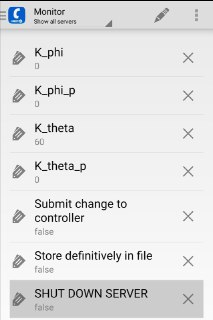
\includegraphics[width=0.3\textwidth]{Immagini/OPC_UA_params.jpg}
	\caption{Parametri impostabili lato client}
	\label{fig:OPCUA_params}
\end{figure}


All'interno dell'Appendice ~\ref{cod:Appendice_opcua}, abbiamo racchiuso in figura ~\ref{fig:OPCUA_diagram}, tramite diagramma di flusso, il funzionamento di massima del codice lato server: codice che siamo andati a testare utilizzando un'apposita app per smartphone Android (\href{https://play.google.com/store/apps/details?id=com.prosysopc.ua.android2&hl=it}{OPC-UA Android client}).

Per quanto riguarda invece l'effettiva implementazione, sempre in Appendice ~\ref{cod:Appendice_opcua}, abbiamo riportato l'intero codice prodotto per la gestione della comunicazione OPC-UA.

\newpage
\section{RTOS - XENOMAI}
\label{sec:xenomai}

Nella parte di controllo di sistemi in generale, risulta essere sempre necessario andare a lavorare in \textit{Real-Time}, ovvero il sistema richiede che il calcolatore sia in grado di produrre computazioni corrette andando allo stesso tempo a rispettare delle \textit{dealine} temporali, ovvero dei vincoli che validano o meno il risultato prodotto.

Come ben noto nall'ambiente informatico, \textit{Linux}, che rappresenta l'\textit{OS} installato a bordo di Raspberry, risulta essere un sistema operativo \textbf{non} \textit{RTOS} (Real Time Operative System): è stato quindi necessario andare ad improntare un aproccio che permesso di renderlo tale.

In questo contesto è risultato essere di fondamentale importanza il software \textit{Xenomai}, un progetto open source creato per fornire un framework real-time per le piattaforme Linux, con l'obbiettivo di aiutare la migrazione di progetti in ambito industriale da sistemi real-time proprietari a sistemi diffusi come Linux.

Il cuore delle funzionalità offerte da Xenomai, sta nella praticità e facilità con cui mette a disposizioni delle API di tipo real-time, occupandosi anche di garantire quelli che sono i limiti e vincoli temporali. 

Di seguito una breve descrizione degli step principali seguiti per quanto concerne la parte di adattamento del controllore Raspberry a RTOS.

\begin{itemize}
	\item Come prima cosa siamo andati a rivedere i files \textit{.cpp} contente la logica di controllo, ritoccando la parte relativa alla lettura dei dati dal file, andando ad utilizzare le API presenti in ambiente c invece di quelle relative a cpp.
	Abbiamo quindi provato e testato la lettura da file tramite il tool DevC++, facilitando così il testing e il debug;
	\item Siamo andati ad installare una macchina virtuale con a bordo \textbf{debian 9.8.0} e la patch \textbf{Xenomai 3.0.8} (\cite{xenomai});
	\item Essendo debian un OS interamente fruibile da linea di comando, siamo andati a prendere confidenza con l'ambiente, cercando di capire l'organizzazione e chiamando gli update/upgrade necessari;
	\item Prima di andare ad importare il file completo (di cui abbiamo parlato al punto iniziale), siamo andati ad eseguire alcuni esempi iniziali (una sorta di HelloWorld):
	\begin{itemize}
		\item Abbiamo per primo cosa studiato questo approccio iniziale (\href{http://www.cs.ru.nl/J.Hooman/DES/XenomaiExercises/Exercise-1.html}{link})
		\item Siamo andati ad impostare il funzionamento di un task (dummy) periodico, come se si trattasse appunto del main loop di un sistema Real-Time;
	\end{itemize}
	
	\item Lo step successivo è stato quello di importare il codice scritto e testato in ambiente DevC++ in Xenomai, provandolo e introducendo alcuni dettagli aggiuntivi, come presentato nei punti seguenti:
	\begin{itemize}
		\item Come primo step risulta essere necessario fornire al framework Xenomai il nome di quale file con estensione .c andare a compilare e successivamente, incapsulare in un framework real-time
			\begin{figure}[H]
				\centering   	
				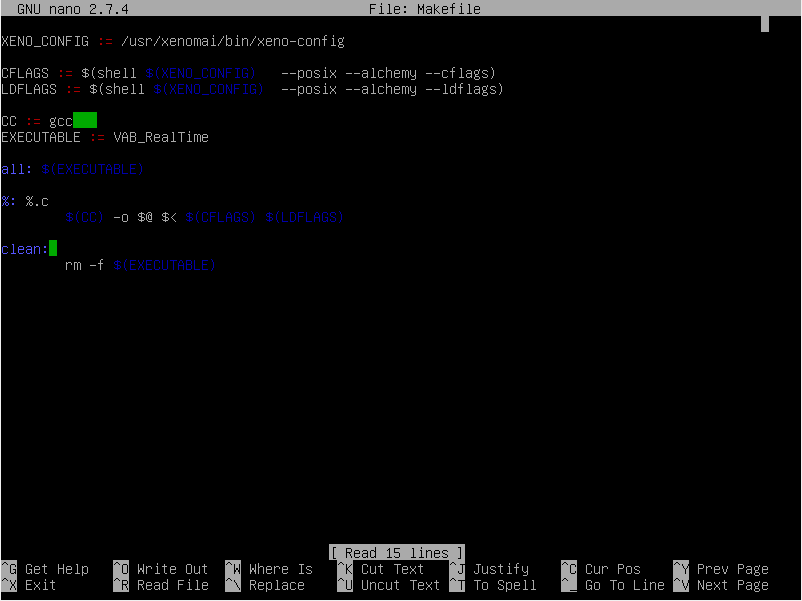
\includegraphics[width=0.6\textwidth]{Immagini/xenomai_nano_make.png}
				\caption{Per specificare quale file \textit{.c} compilare}
				\label{fig:xenomai_nano_make}
			\end{figure}
		\item Abbiamo specificato quello che è il periodo di funzionamento  tramite i seguenti comandi:
		\begin{lstlisting}
		RTIME period  = 1000000000; % Expressed in [ns]
		rt_task_set_periodic(NULL,TM_NOW,period);
		\end{lstlisting}
		
		\item All'interno del ciclo while, abbiamo definito un continuo update dei parametri temporali di nostro interesse.
		
		Nello specifico ad inizio ciclo andiamo a sovrascrivere constantemente il parametro \textit{now} mentre, nella parte finale del ciclo stesso, abbiamo impostato un update del parametro \textit{before}.
		
		Il salvataggio di queste variabili permette di facilitare, in qualsiasi punto del codice, l'accesso ai parametri temporali per eventuali necessità di calcolo, come nella definizione dell'intervallo di tempo su cui andare a realizzare i vari calcoli derivativi necessari per il corretto controllo;
		\begin{figure}[H]
			\centering   	
			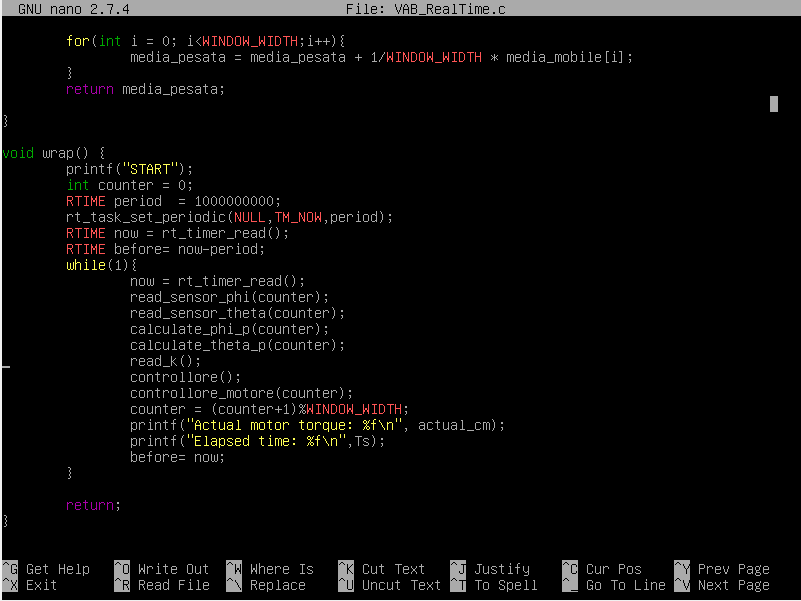
\includegraphics[width=0.8\textwidth]{Immagini/xenomai_nano.png}
			\caption{Definizione e temporizzazione del ciclo \textit{WHILE}}
			\label{fig:xenomai_nano}
		\end{figure}
		\item Come si vede anche in figura ~\ref{fig:xenomai_nano}, nel ciclo principale abbiamo messo in successione questi blocchi (eseguiti a frequenza fissa): 
		\begin{itemize}
			\item Lettura dei parametri da files;
			\item Lettura dei valori misurati della parte sensoristica;
			\item Elaborazione dei dati rilevati e algoritmo di controllo;
			\item Produzione dei risultati di interesse
		\end{itemize}
		\item In figura ~\ref{fig:xenomai_execution} si può vedere come, ogni ciclo di lettura del file con i parametri, che corrisponde ad un ciclo macchina, presenti un tempo fisso.
		
		Infatti, con il termine \textit{"Elapsed time"} siamo andati a stampare il \textit{delta} temporale, il quale rappresenta il tempo occupato da un singolo ciclo macchina;
		\begin{figure}[H]
			\centering   	
			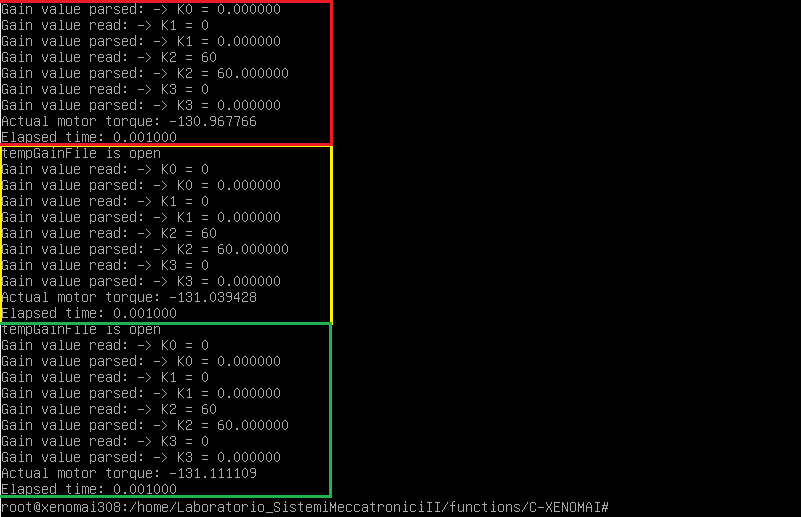
\includegraphics[width=0.8\textwidth]{Immagini/xenomai_execution.png}
			\caption{Esecuzione a tempo fissato  (1 ms) delle funzioni di lettura e calcolo}
			\label{fig:xenomai_execution}
		\end{figure}
		\item La gestione del thread relativo al server \textit{OPC-UA} non è ancora stato gestito: esso sarà ovviamente lasciato in secondo piano rispetto al thread di lavoro principale principale temporizzato alla frequenza specifica;
	\end{itemize}
\end{itemize}